\begingroup
\fontencoding{T5}\selectfont
\section{Implementation}
\subsection{User Interface Design for Authentication Module}

The Authentication Module serves as the primary gateway for system access across all user roles in the BkLib Online Library Management System. It enforces secure identity verification, role-based entry routing, self-service user onboarding, and a multi-step password recovery workflow.

\paragraph{Login Page}
Primary entry portal providing unified authentication with role-switching tabs.

\begin{figure}[H]
    \centering
    
\includegraphics[width=0.95\linewidth]{Images/Auth_DangNhap.png}
    \vspace{10pt}
    \caption{BkLib Login Interface}
    \label{fig:auth_login}
\end{figure}

\textbf{Layout \& Functionality:} Features a split-screen layout with branding artwork on the left and a clean authentication card on the right. Includes a role selector tab ("Bạn đọc / Sinh viên" vs. "Cán bộ / Quản trị"), credentials input fields (email or username, password with visibility toggle), a "Ghi nhớ đăng nhập" (Remember Me) checkbox, and direct triggers for password recovery ("Quên mật khẩu?") and account registration. Upon validation, users are automatically routed to their designated workspace.

\paragraph{Registration Page}
Self-service onboarding page for new library members to register accounts with branch selection.

\begin{figure}[H]
    \centering
    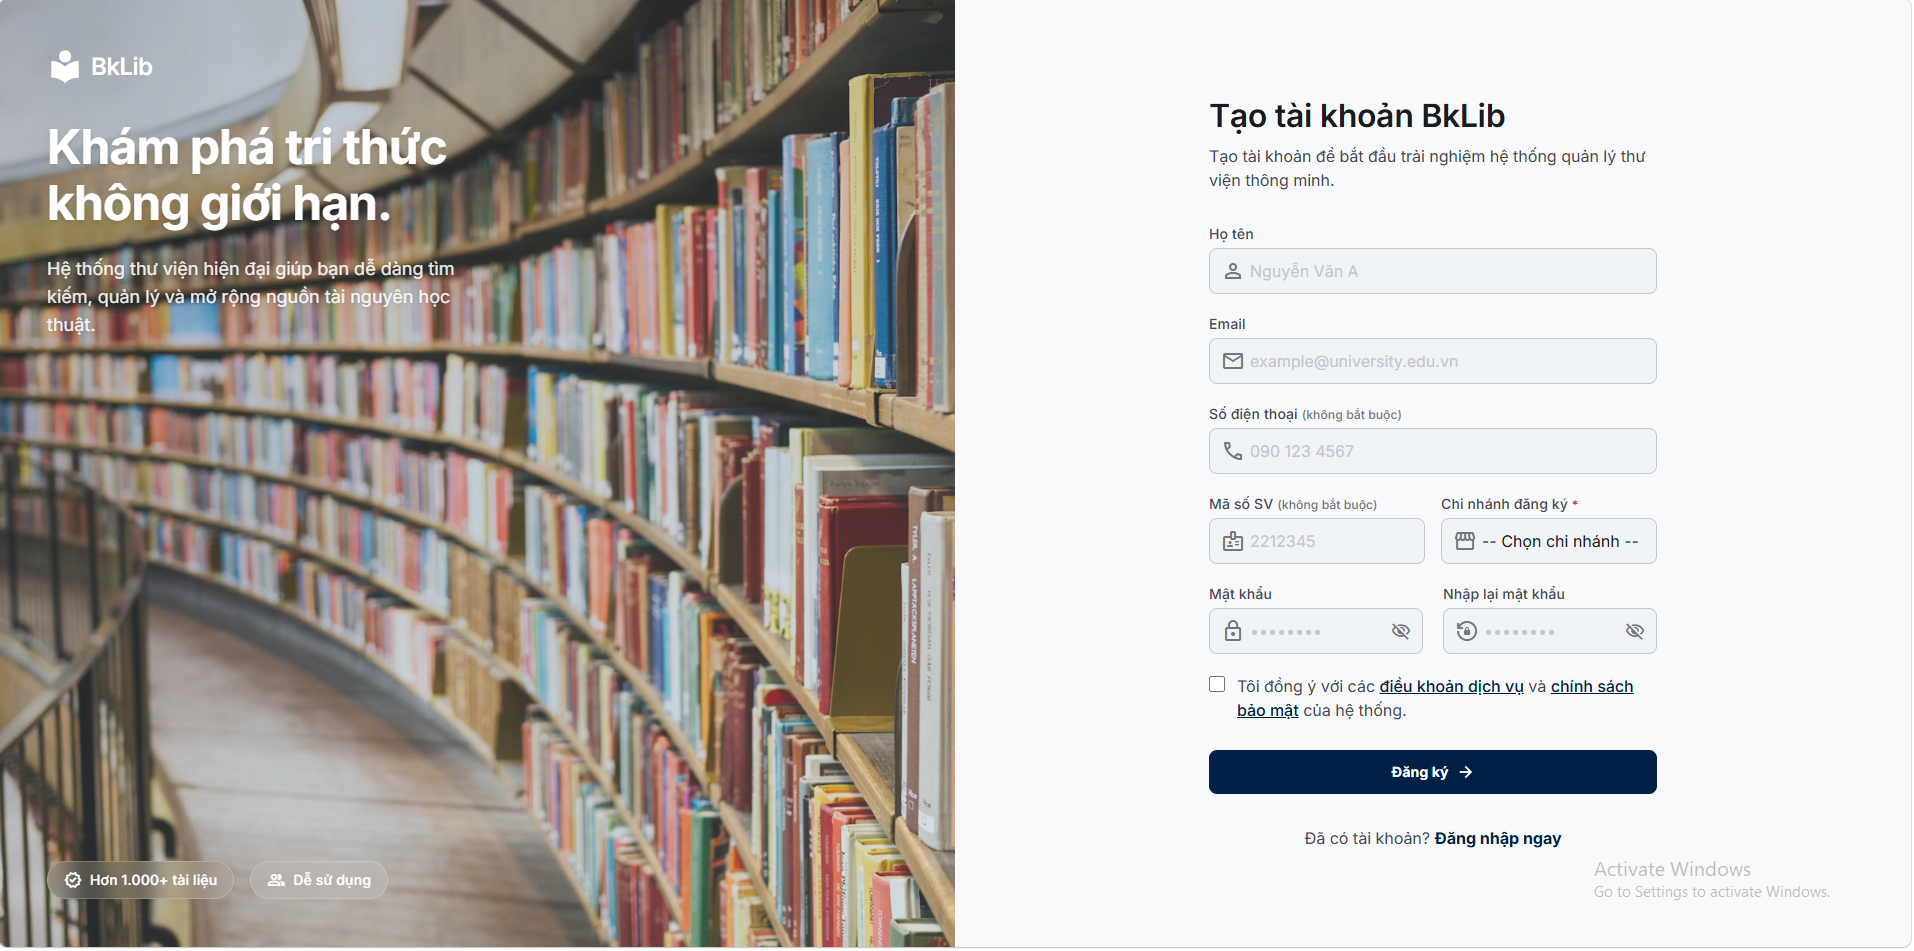
\includegraphics[width=0.95\linewidth]{Images/Auth_DangKy.png}
    \vspace{10pt}
    \caption{BkLib Account Registration Interface}
    \label{fig:auth_register}
\end{figure}

\textbf{Layout \& Functionality:} Structured form capturing essential user profile details, including Full Name, Email, Phone Number (optional), Student ID ("Mã số SV" - optional), and Branch Selection ("Chi nhánh đăng ký"). It mandates password creation with confirmation matching and terms of service consent ("Điều khoản dịch vụ" and "Chính sách bảo mật") prior to submitting the registration request.

\paragraph{Password Reset Workflow (3-Step Modal)}
Modal-based self-service credential recovery mechanism utilizing 6-digit Email OTP verification.

\begin{figure}[H]
    \centering
    \begin{subfigure}[b]{0.32\textwidth}
        \centering
        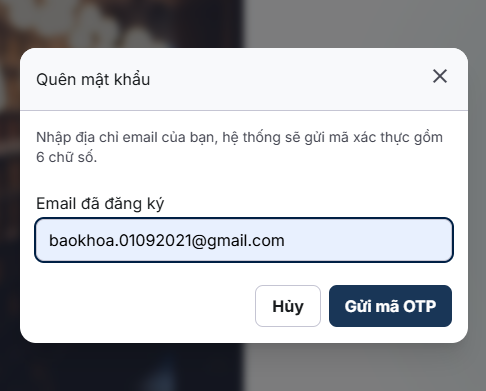
\includegraphics[width=\textwidth]{Images/Auth_QuenMatKhau_B1.png}
        \caption{Step 1: Email Submission}
        \label{fig:auth_reset_step1}
    \end{subfigure}
    \hfill
    \begin{subfigure}[b]{0.32\textwidth}
        \centering
        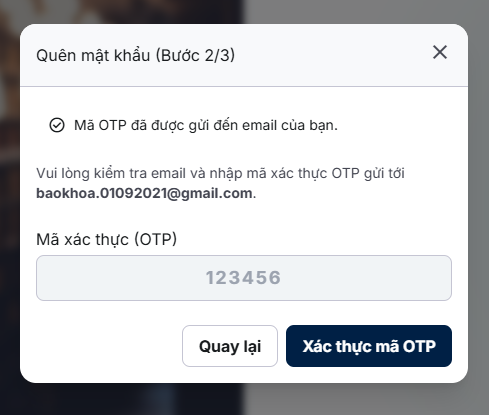
\includegraphics[width=\textwidth]{Images/Auth_QuenMatKhau_B2.png}
        \caption{Step 2: OTP Verification}
        \label{fig:auth_reset_step2}
    \end{subfigure}
    \hfill
    \begin{subfigure}[b]{0.32\textwidth}
        \centering
        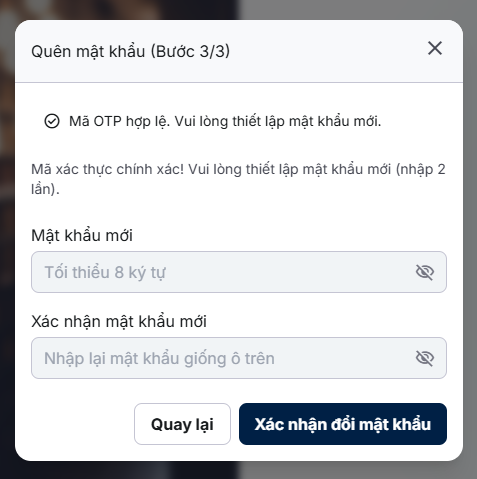
\includegraphics[width=\textwidth]{Images/Auth_QuenMatKhau_B3.png}
        \caption{Step 3: Password Reset}
        \label{fig:auth_reset_step3}
    \end{subfigure}
    \vspace{10pt}
    \caption{Three-step Modal Workflow for Password Recovery}
    \label{fig:auth_forgot_password_flow}
\end{figure}

\textbf{Layout \& Functionality:} Executes within an overlay modal dialog spanning three sequential stages:
\begin{itemize}
    \item \textbf{Step 1 (Request OTP):} Users enter their registered email address to dispatch a 6-digit verification code.
    \item \textbf{Step 2 (OTP Verification):} Prompts input of the 6-digit code received via email, featuring validation feedback and back-navigation controls.
    \item \textbf{Step 3 (Password Update):} Prompts creation and confirmation of a new password (minimum 8 characters) with eye icons for masked text toggling.
\end{itemize}

\subsection{User Interface Design for Reader Module}

The Reader Module provides self-service capabilities for library patrons. It enables authenticated readers to browse the catalog, execute semantic AI-powered resource searches, track and renew active loans, monitor hold queue statuses, view historical borrowing transactions, and update personal notification settings.

\paragraph{Homepage}
Personalized central dashboard rendered upon reader authentication, serving as the operational hub for patron activities.

\begin{figure}[H]
    \centering
    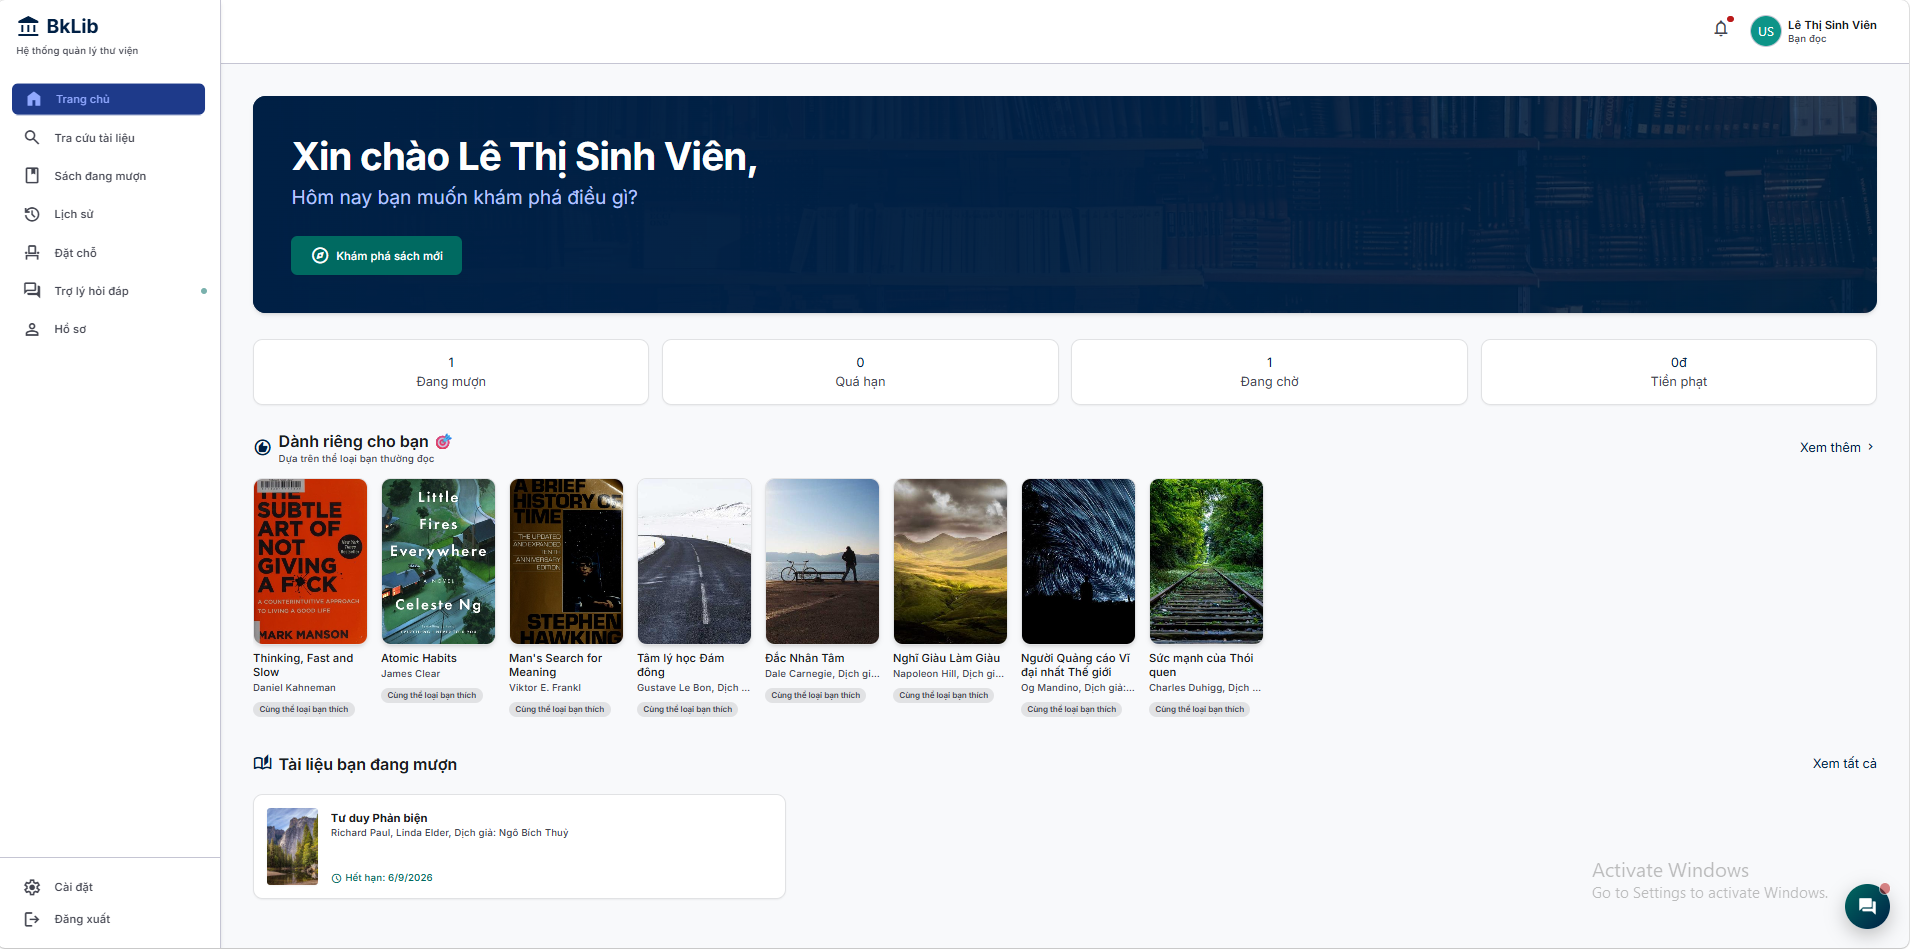
\includegraphics[width=0.95\linewidth]{Images/Reader_TrangChu.png}
    \vspace{10pt}
    \caption{Reader Module Homepage Interface}
    \label{fig:reader_homepage}
\end{figure}

\textbf{Layout \& Functionality:} Includes a responsive left navigation sidebar, top notification center, key metric summary cards (active loans, overdue items, active holds, fine balances), and quick-access cards for currently borrowed books with real-time due date indicators.

\paragraph{Catalog Search Page}
Interface for discovery, multi-criteria filtering, and digital resource catalog browsing.

\begin{figure}[H]
    \centering
    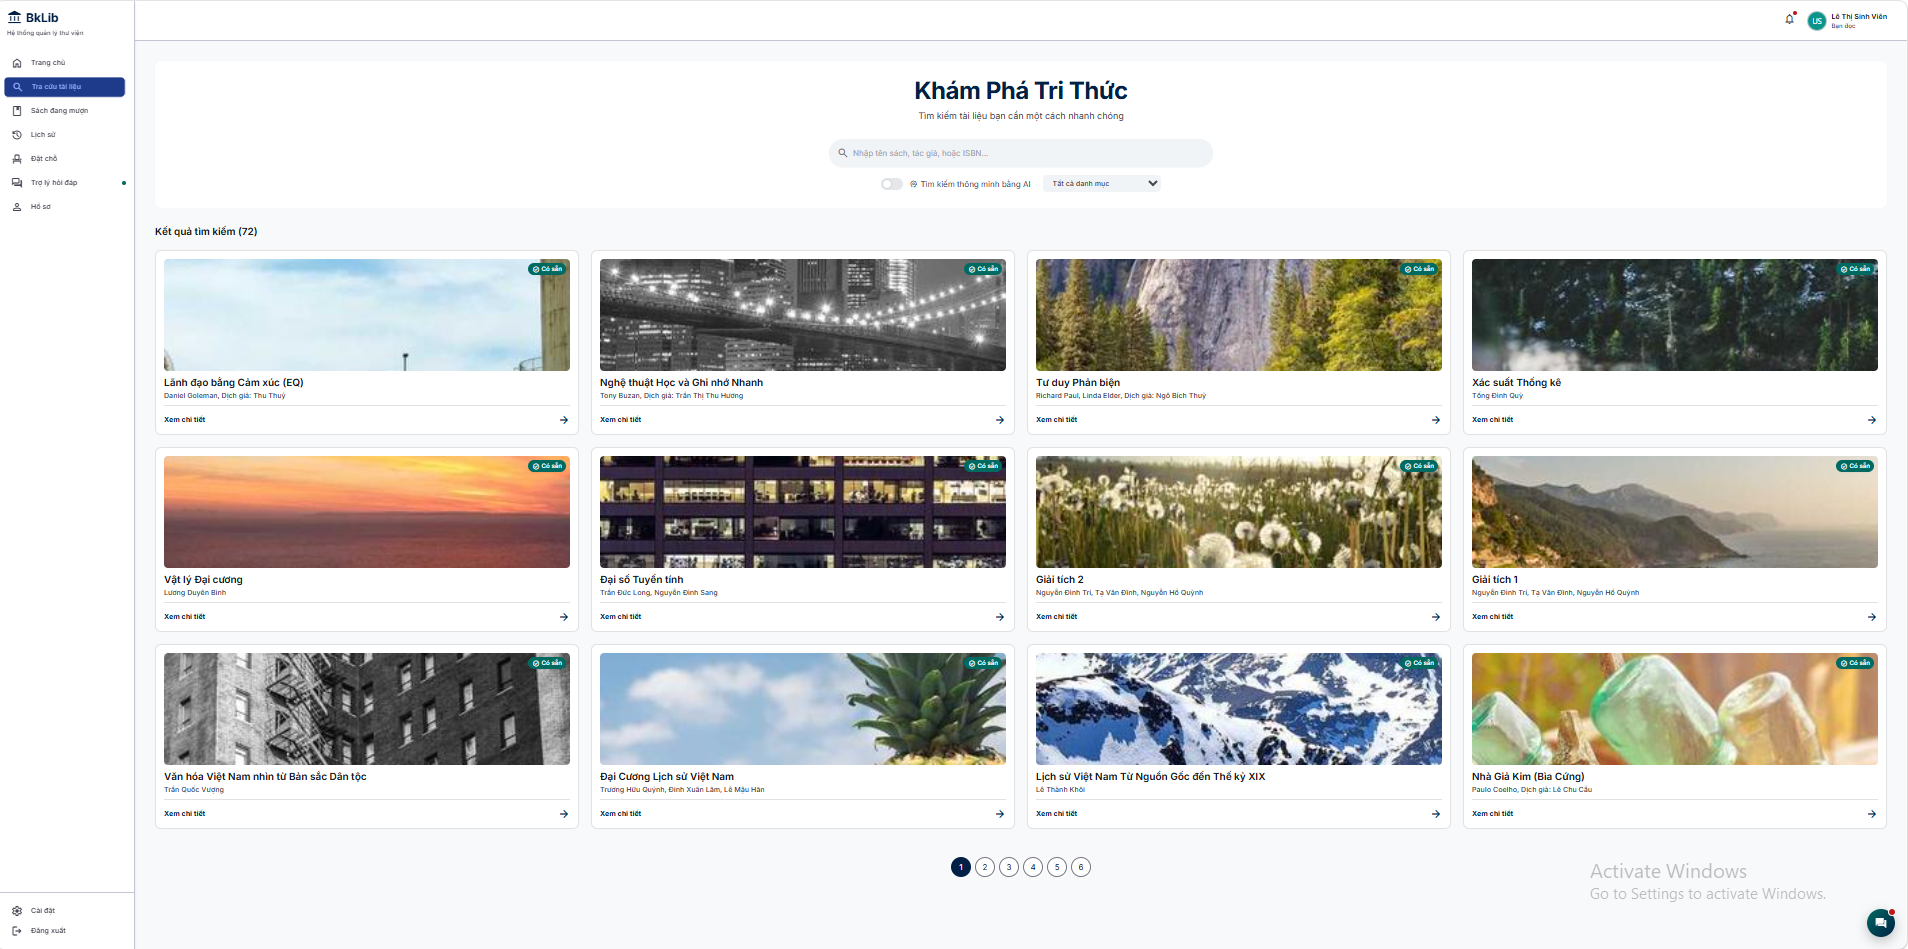
\includegraphics[width=0.95\linewidth]{Images/Reader_TraCuu.png}
    \vspace{10pt}
    \caption{Catalog Search Interface}
    \label{fig:reader_search}
\end{figure}

\textbf{Layout \& Functionality:} Integrates an advanced keyword search bar with category and branch availability filters. Readers can view cover imagery, metadata (author, publisher, ISBN), real-time availability status, and initiate physical hold reservations directly from search result cards.

\paragraph{Active Loans Management Page}
Dedicated view allowing readers to monitor loan lifecycles and trigger online loan renewals.

\begin{figure}[H]
    \centering
    
\includegraphics[width=0.95\linewidth]{Images/Reader_SachDangMuon.png}
    \vspace{10pt}
    \caption{Active Loans Management Interface}
    \label{fig:reader_borrowing}
\end{figure}

\textbf{Layout \& Functionality:} Displays loan summary statistics alongside detailed item cards indicating checkout dates, mandatory due dates, and renewal attempt limits. Readers can execute inline renewals, which dynamically query circulation rules to recalculate due dates or flag renewal constraints (e.g., existing holds or maximum extension limits).

\paragraph{Loan History Page}
Historical ledger recording past transactions, returned items, and financial interactions.

\begin{figure}[H]
    \centering
    
\includegraphics[width=0.95\linewidth]{Images/Reader_LichSu.png}
    \vspace{10pt}
    \caption{Loan History Interface}
    \label{fig:reader_history}
\end{figure}

\textbf{Layout \& Functionality:} Structured table containing book titles, checkout dates, actual return timestamps, fulfillment status badges, and assessed fine records. Features client-side column sorting and date-range filter triggers for personal record auditing.

\paragraph{Active Holds Page}
Monitors reservation queue positions and availability notices for out-of-stock items.

\begin{figure}[H]
    \centering
    
\includegraphics[width=0.95\linewidth]{Images/Reader_DatCho.png}
    \vspace{10pt}
    \caption{Active Holds Interface}
    \label{fig:reader_reservation}
\end{figure}

\textbf{Layout \& Functionality:} Lists active reservations with queue ordering, expiration windows for ready-for-pickup notifications, cancel hold triggers, and an informational panel detailing library reservation rules and pickup deadlines.

\paragraph{Virtual Assistant Chat Window}
Interactive AI assistant widget facilitating natural language interaction, QA, and semantic recommendation.

\begin{figure}[H]
    \centering
    
\includegraphics[width=0.45\linewidth]{Images/Reader_ChatbotAI.png}
    \vspace{10pt}
    \caption{Virtual Assistant Chat Window Interface}
    \label{fig:reader_chatbot}
\end{figure}

\textbf{Layout \& Functionality:} Floating chat interface utilizing a hybrid Retrieval-Augmented Generation (RAG) backend. Features prompt suggestions, streaming response bubble threads, and direct deep-links to catalog book details generated from semantic similarity queries.

\paragraph{Personal Profile \& Settings Page}
Patron account management, security credentials, and communication preferences.

\begin{figure}[H]
    \centering
    
\includegraphics[width=0.95\linewidth]{Images/Reader_HoSoCaiDat.png}
    \vspace{10pt}
    \caption{Personal Profile and Settings Interface}
    \label{fig:reader_profile}
\end{figure}

\textbf{Layout \& Functionality:} Contains editable personal contact forms, password modification tools, multi-channel notification toggles (Email, SMS, In-App), and a personalized recommendation grid driven by patron reading history.

\subsection{User Interface Design for Librarian Module}

The Librarian Module empowers library staff to manage daily counter operations, oversee item circulation, maintain catalog metadata, communicate system announcements, and analyze branch performance analytics.

\paragraph{Homepage}
Operational control panel highlighting daily tasks, branch status indicators, and urgent action queues.

\begin{figure}[H]
    \centering
    
\includegraphics[width=0.95\linewidth]{Images/Librarian_TrangChu.png}
    \vspace{10pt}
    \caption{Librarian Module Homepage Interface}
    \label{fig:librarian_homepage}
\end{figure}

\textbf{Layout \& Functionality:} Features quick-action navigation shortcuts (Circulation, Cataloging, Announcements, Reports), real-time counter performance metrics, pending reservation queues awaiting processing, and an activity log feed tracking recent loan activities.

\paragraph{Circulation Management Page}
Counter processing interface engineered for high-throughput checkouts, returns, and fine settlement.

\begin{figure}[H]
    \centering
    
\includegraphics[width=0.95\linewidth]{Images/Librarian_QuanLyLuuThong.png}
    \vspace{10pt}
    \caption{Circulation Management Interface}
    \label{fig:librarian_circulation}
\end{figure}

\textbf{Layout \& Functionality:} Dual-pane interface: Patron ID/barcode lookup pane on the left, and rapid barcode scanning input area with active transaction summary and item return validation on the right. Instantly verifies patron account status, overdue holds, and automatic fine calculation upon scanning.

\paragraph{Catalog Management Page}
Administrative workspace for book metadata management, inventory tracking, and physical copy labeling.

\begin{figure}[H]
    \centering
    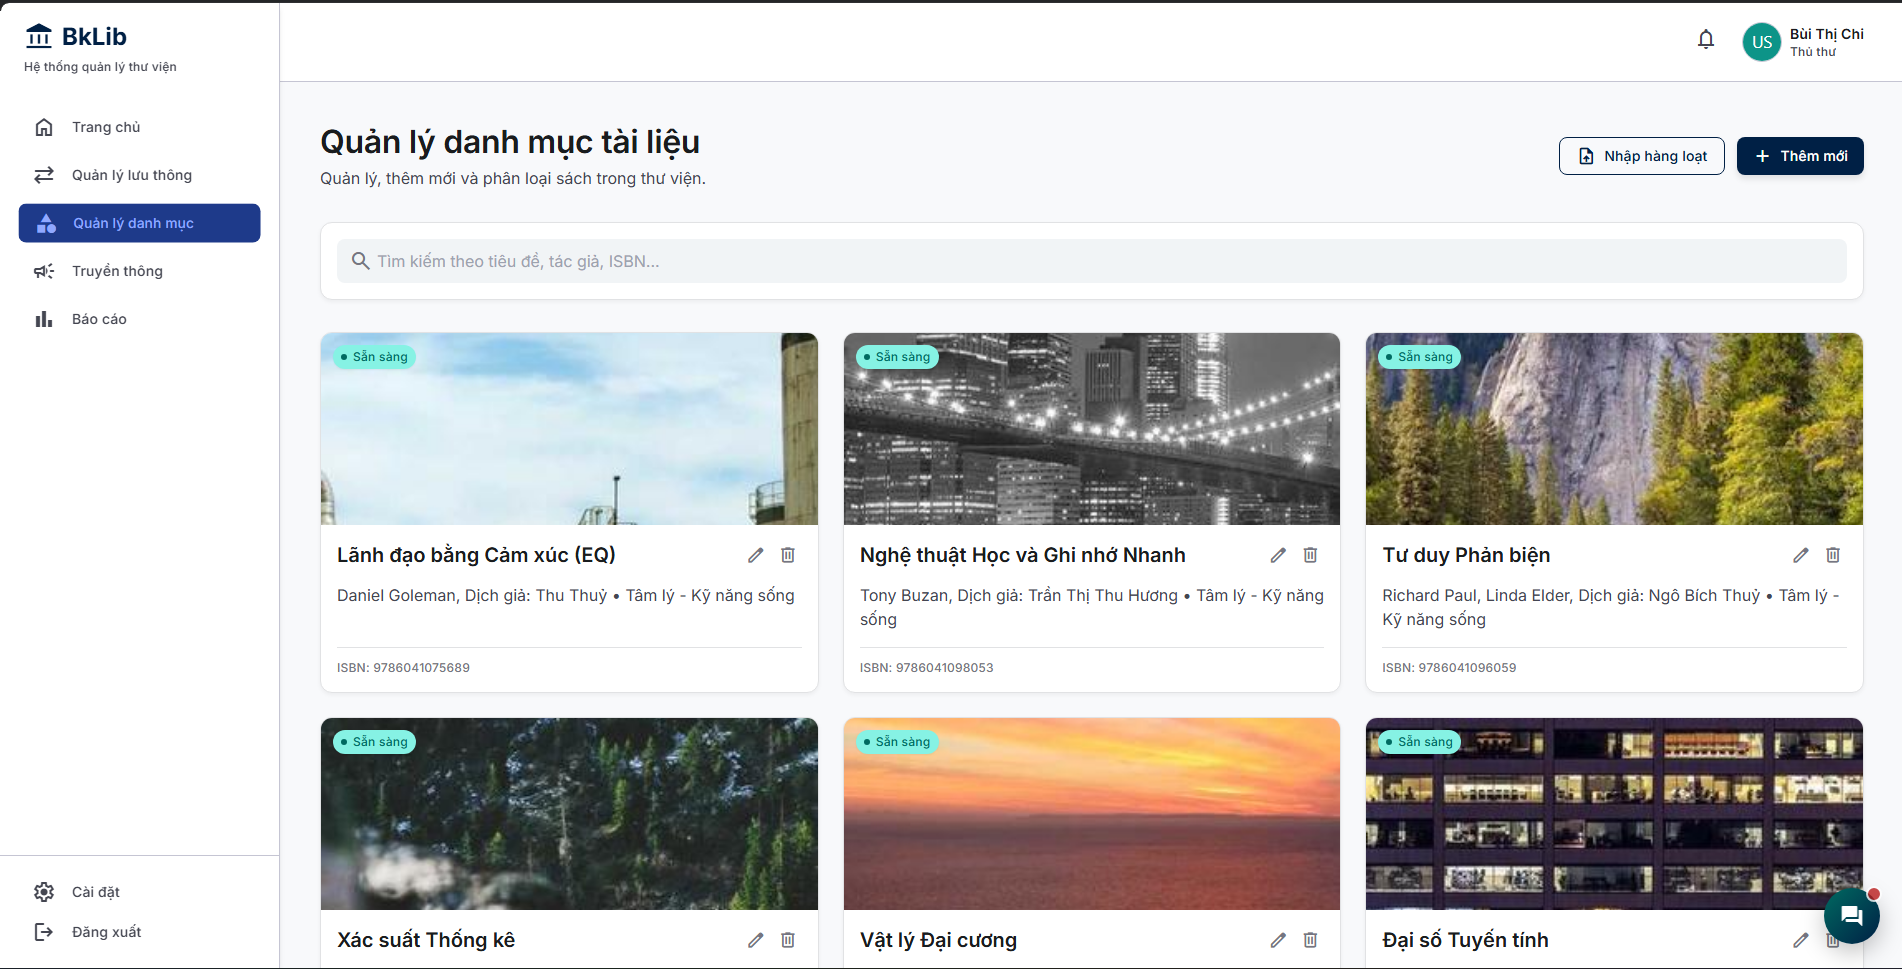
\includegraphics[width=0.95\linewidth]{Images/Librarian_QuanLyDanhMuc.png}
    \vspace{10pt}
    \caption{Catalog Management Interface}
    \label{fig:librarian_catalog}
\end{figure}

\textbf{Layout \& Functionality:} Search control bar with ISBN auto-fetching integration, batch CSV/Excel import tools, item modal creation form, and a paginated inventory table providing inline record editing, status toggling, and copy barcode generation.

\paragraph{Communication Management Page}
Broadcast dispatch portal for library announcements and target reader notification campaigns.

\begin{figure}[H]
    \centering
    
\includegraphics[width=0.95\linewidth]{Images/Librarian_TruyenThong.png}
    \vspace{10pt}
    \caption{Communication Management Interface}
    \label{fig:librarian_notification}
\end{figure}

\textbf{Layout \& Functionality:} Rich-text announcement composition editor with audience targeting options (All Readers, Overdue Borrowers, Specific Member Tiers), channel selection (In-App, Email), and a historical broadcast log detailing delivery success rates.

\paragraph{Reports \& Analytics Page}
Data visualization dashboard tracking circulation throughput, collection usage, and financial metrics.

\begin{figure}[H]
    \centering
    
\includegraphics[width=0.95\linewidth]{Images/Librarian_BaoCao.png}
    \vspace{10pt}
    \caption{Librarian Reports and Analytics Interface}
    \label{fig:librarian_report}
\end{figure}

\textbf{Layout \& Functionality:} Interactive date-range controls, export triggers (PDF, Excel, CSV), circulation trend charts, top-borrowed book rankings, and fine collection breakdowns to assist inventory planning.

\paragraph{Personal Profile \& Settings Page}
Staff account management workspace for updating staff profile attributes, security credentials, and system notification preferences.

\begin{figure}[H]
    \centering
    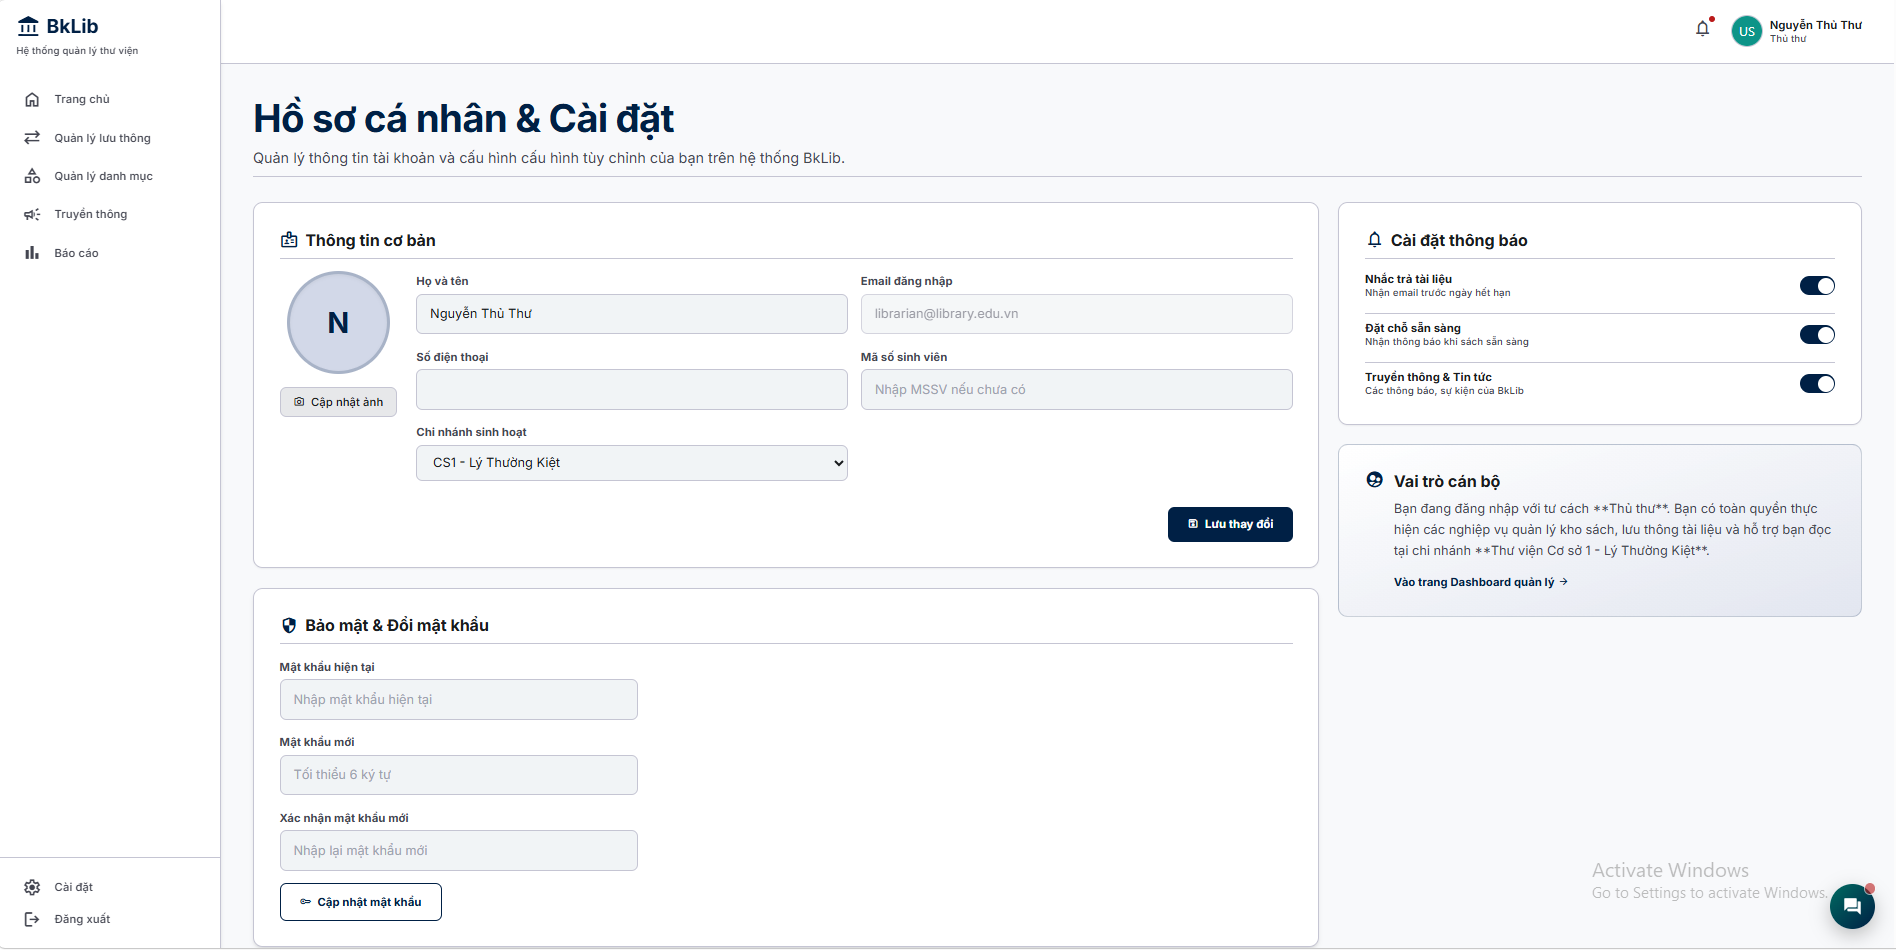
\includegraphics[width=0.95\linewidth]{Images/Librarian_HoSoCaiDat.png}
    \vspace{10pt}
    \caption{Librarian Personal Profile and Settings Interface}
    \label{fig:librarian_profile}
\end{figure}

\textbf{Layout \& Functionality:} Organized into a multi-card dashboard layout:
\begin{itemize}
    \item \textbf{Basic Information Pane ("Thông tin cơ bản"):} Editable profile fields including full name, login email, contact phone number, student/staff ID, assigned operating branch selector (e.g., CS1 - Lý Thường Kiệt), and profile avatar update controls.
    \item \textbf{Security \& Password Modification ("Bảo mật \& Đổi mật khẩu"):} Password management utility requiring current password verification followed by new password entry and confirmation matching.
    \item \textbf{Notification Preferences ("Cài đặt thông báo"):} Granular toggle switches for key automated alerts, including document return reminders, hold availability notifications, and system-wide announcements.
    \item \textbf{Staff Role Summary Panel ("Vai trò cán bộ"):} Informational context card detailing current authorization privileges, assigned operational branch scope, and a direct navigation link to the administrative dashboard.
\end{itemize}

\subsection{User Interface Design for Administrator Module}

The Administrator Module provides top-level governance for platform management. It enables system administrators to manage Role-Based Access Control (RBAC), configure branch network settings, audit system logs, monitor infrastructure health, and control disaster recovery procedures.

\paragraph{System Overview Dashboard}
High-level system health dashboard monitoring infrastructure resources, server loads, and usage statistics.

\begin{figure}[H]
    \centering
    
\includegraphics[width=0.95\linewidth]{Images/Admin_Dashboard.png}
    \vspace{10pt}
    \caption{Administrator System Overview Dashboard}
    \label{fig:admin_dashboard}
\end{figure}

\textbf{Layout \& Functionality:} Displays system metrics cards (Total Active Accounts, Catalog Size, Active Sessions), cloud database storage indicators, API traffic throughput graphs, and real-time system security alerts.

\paragraph{User Account Management Page}
Centralized administration workspace for user identity lifecycle, role assignments, and permission management.

\begin{figure}[H]
    \centering
    
\includegraphics[width=0.95\linewidth]{Images/Admin_QuanLyTaiKhoan.png}
    \vspace{10pt}
    \caption{User Account Management Interface}
    \label{fig:admin_user_management}
\end{figure}

\textbf{Layout \& Functionality:} Paginated user directory with role-based filtering (Reader, Librarian, Admin), account creation modal trigger, RBAC permission assignment controls, and emergency account lock/unlock toggles.

\paragraph{System Configuration Page}
Centralized administrative interface for defining operational system parameters, circulation rules, and fine structures.

\begin{figure}[H]
    \centering
    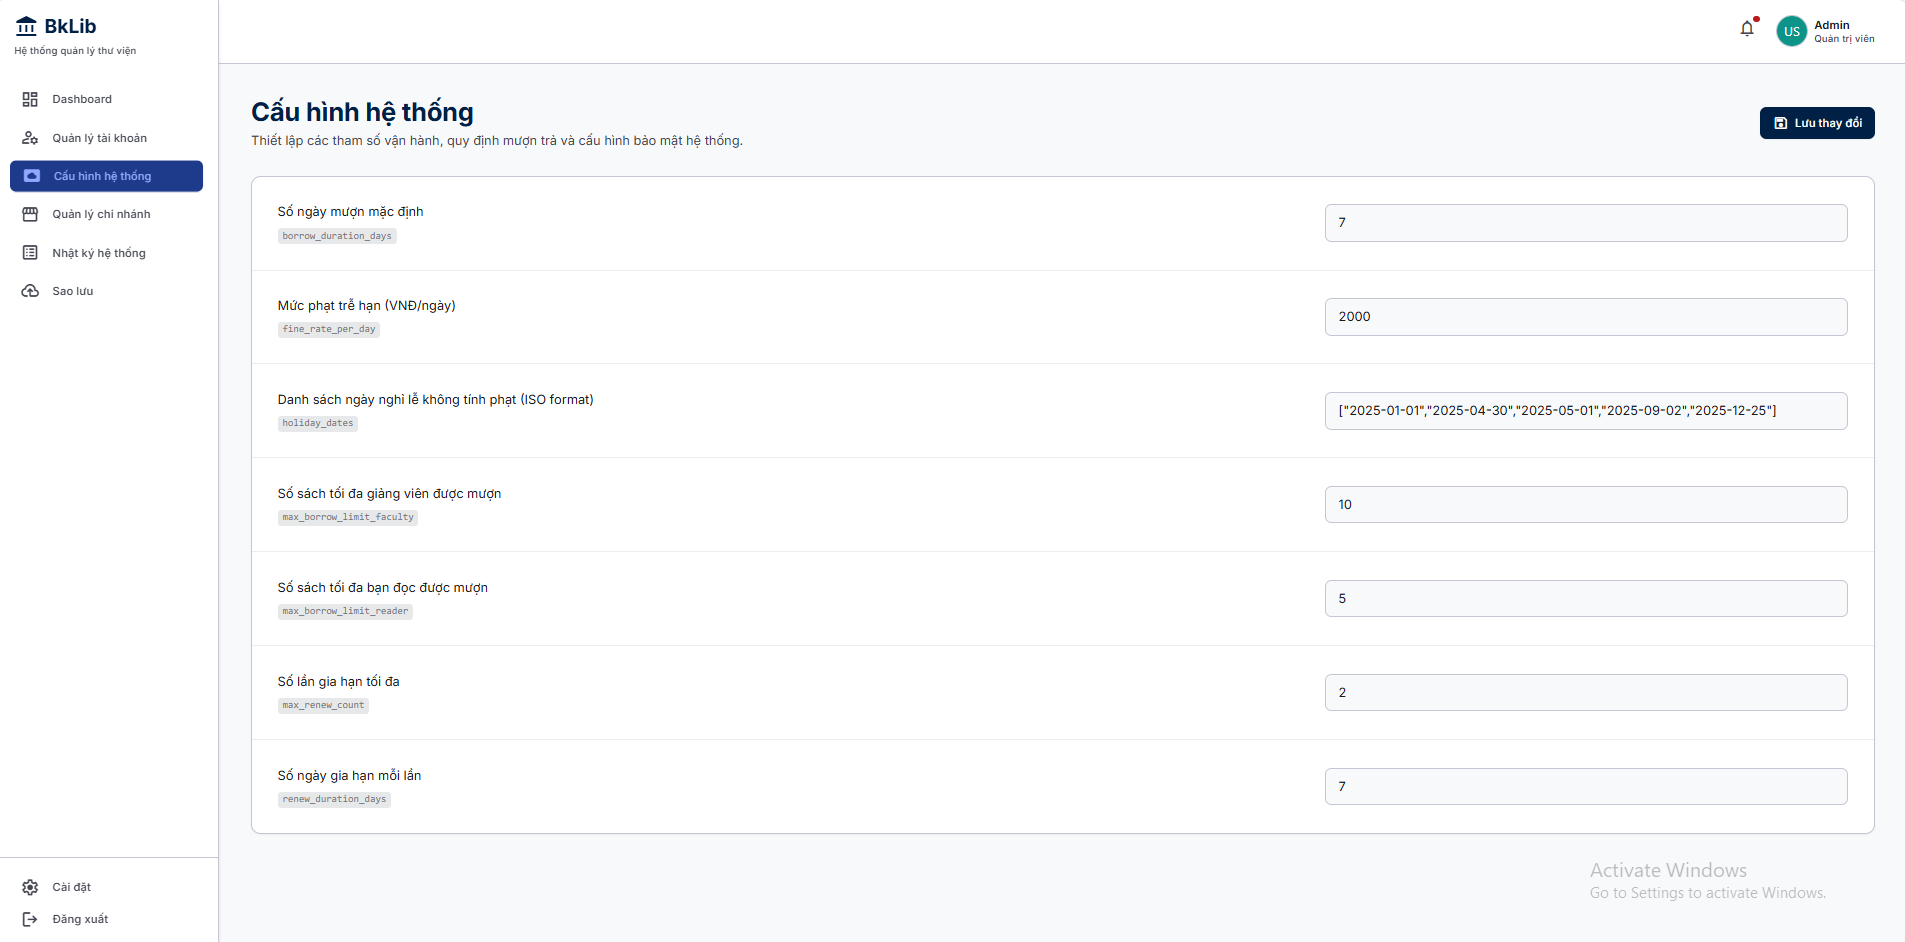
\includegraphics[width=0.95\linewidth]{Images/Admin_CauHinhHeThong.png}
    \vspace{10pt}
    \caption{System Configuration Interface}
    \label{fig:admin_system_config}
\end{figure}

\textbf{Layout \& Functionality:} Structured configuration panel providing interactive inputs for global system environment variables, including:
\begin{itemize}
    \item \textbf{Circulation Rules:} Default borrowing duration in days (\texttt{borrow\_duration\_days}), max borrowing limit for faculty members (\texttt{max\_borrow\_limit\_faculty}), and general reader borrowing cap (\texttt{max\_borrow\_limit\_reader}).
    \item \textbf{Renewal Policies:} Maximum allowable renewals per item (\texttt{max\_renew\_count}) and duration granted per renewal cycle (\texttt{renew\_duration\_days}).
    \item \textbf{Financial \& Calendar Settings:} Daily overdue fine rate calculation in VNĐ (\texttt{fine\_rate\_per\_day}) and an array-formatted holiday exclusion list (\texttt{holiday\_dates}) in ISO format to suspend fine accruals during non-working days.
\end{itemize}

\paragraph{Branch Management Page}
Network topology configuration page for physical library branches and inter-branch policies.

\begin{figure}[H]
    \centering
    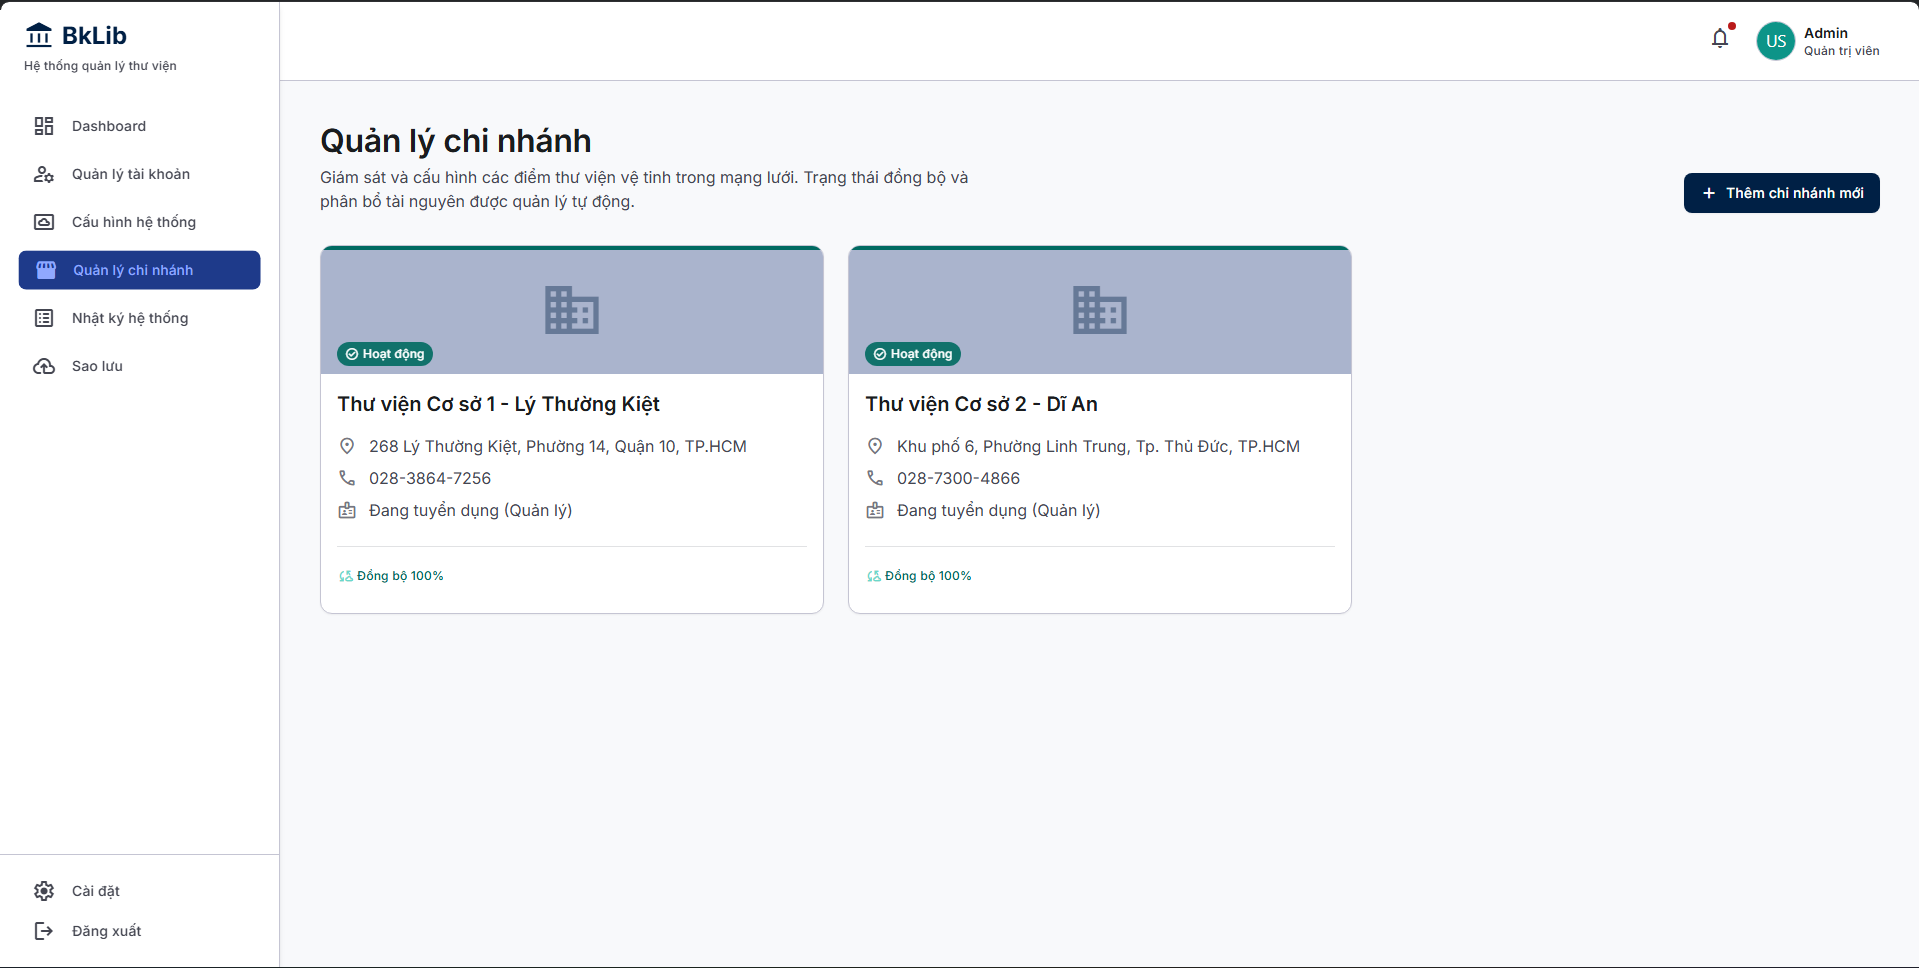
\includegraphics[width=0.95\linewidth]{Images/Admin_QuanLyChiNhanh.png}
    \vspace{10pt}
    \caption{Branch Management Interface}
    \label{fig:admin_branch_management}
\end{figure}

\textbf{Layout \& Functionality:} Grid of branch profile cards displaying branch addresses, contact details, assigned head librarians, operating hours, and synchronization status with the central database.

\paragraph{Audit Logs Page}
Compliance and security audit trail viewer logging critical system actions and data state mutations.

\begin{figure}[H]
    \centering
    
\includegraphics[width=0.95\linewidth]{Images/Admin_NhatKyKiemToan.png}
    \vspace{10pt}
    \caption{System Audit Logs Interface}
    \label{fig:admin_audit_log}
\end{figure}

\textbf{Layout \& Functionality:} High-density audit event table detailing action timestamps, actor identities and IP addresses, API endpoint paths, before/after JSON payload diffs, and severity badges for anomaly tracking.

\paragraph{Backup \& Disaster Recovery Page}
Database snapshot management and disaster recovery administration tool.

\begin{figure}[H]
    \centering
    
\includegraphics[width=0.95\linewidth]{Images/Admin_SaoLuuPhucHoi.png}
    \vspace{10pt}
    \caption{Backup and Disaster Recovery Interface}
    \label{fig:admin_backup}
\end{figure}

\textbf{Layout \& Functionality:} Displays automated backup scheduling configurations, snapshot storage usage, manual immediate backup trigger controls, historical snapshot logs, and point-in-time database restoration controls.

\subsection{Core Technical Implementation Highlights}

To complement the user interface design, this section details the backend implementation mechanisms and core algorithm logic powering key system functionalities across security, circulation policies, AI retrieval, and audit governance.

\subsubsection{Role-Based Access Control (RBAC) \& JWT Authentication}
Security and endpoint protection are enforced through middleware leveraging JSON Web Tokens (JWT) and a higher-order role authorization function.

\begin{lstlisting}[caption={JWT Authentication and Authorization Middleware (backend-express/src/middlewares/auth.middleware.ts)}, label={lst:auth_middleware}]
// Middleware verifying JWT access token from Authorization header
export const authenticate = (req: Request, res: Response, next: NextFunction): void => {
  const authHeader = req.headers.authorization;
  if (!authHeader || !authHeader.startsWith('Bearer ')) {
    res.status(401).json({ success: false, message: 'No authorization token provided' });
    return;
  }
  const token = authHeader.split(' ')[1];
  try {
    const decoded = jwt.verify(token, env.JWT_SECRET) as AuthPayload;
    req.user = decoded;
    next();
  } catch (err) {
    res.status(401).json({ success: false, message: 'Invalid or expired token' });
  }
};

// Middleware factory restricting access to specified roles
export const authorize = (...roles: Role[]) => {
  return (req: Request, res: Response, next: NextFunction): void => {
    if (!req.user || !roles.includes(req.user.role)) {
      res.status(403).json({ success: false, message: 'Access denied' });
      return;
    }
    next();
  };
};
\end{lstlisting}

\subsubsection{Dynamic Overdue Penalty \& Holiday Exclusion Calculation}
Circulation logic dynamically calculates overdue days by iterating through loan return intervals while excluding official library holiday dates configured in system settings.

\begin{lstlisting}[caption={Holiday-Aware Overdue Day Calculation (backend-express/src/modules/circulation/circulation.service.ts)}, label={lst:calc_overdue}]
const calcOverdueDays = async (dueDate: Date, returnDate: Date): Promise<number> => {
  if (returnDate <= dueDate) return 0;

  // Retrieve holiday array from system configuration
  const holidayConfig = await getConfig(CONFIG_KEYS.HOLIDAY_DATES, '[]');
  const holidays: string[] = JSON.parse(holidayConfig);

  let overdueDays = 0;
  const cursor = new Date(dueDate);
  cursor.setDate(cursor.getDate() + 1);

  // Iterate day-by-day excluding scheduled holidays
  while (cursor <= returnDate) {
    const dateStr = cursor.toISOString().split('T')[0];
    if (!holidays.includes(dateStr)) {
      overdueDays++;
    }
    cursor.setDate(cursor.getDate() + 1);
  }
  return overdueDays;
};
\end{lstlisting}

\subsubsection{RAG Vector Context Retrieval for AI Assistant}
The Virtual Assistant utilizes vector embeddings generated via \texttt{SentenceTransformer} and stored in an in-memory \texttt{ChromaDB} collection to retrieve top context chunks for patron inquiries.

\begin{lstlisting}[language=Python, caption={ChromaDB Vector Retrieval for RAG (ai-service/app/services/rag\_service.py)}, label={lst:rag_retrieval}]
def retrieve_context(query: str, top_k: int = 3) -> str:
    """
    Retrieve top-k relevant text chunks for a query from ChromaDB vector collection.
    Formats results with segment headers to feed into LLM prompt context.
    """
    if _collection is None or _collection.count() == 0:
        return ""

    embedder = get_embeddings()
    query_embedding = embedder.encode([query]).tolist()

    results = _collection.query(
        query_embeddings=query_embedding,
        n_results=min(top_k, _collection.count()),
    )
    docs = results.get("documents", [[]])[0]
    if not docs:
        return ""

    return "\n\n---\n\n".join([f"[Chunk {i+1}]: {doc}" for i, doc in enumerate(docs)])
\end{lstlisting}

\subsubsection{System Audit Trail \& Change Tracking}
System administrative mutations (such as system configuration adjustments, database backups, or account updates) automatically log immutable audit trail records containing actor metadata and action parameters.

\begin{lstlisting}[caption={Audit Logging Execution (backend-express/src/modules/admin/admin.service.ts)}, label={lst:audit_log}]
await prisma.auditLog.create({
  data: {
    actorId: processedById,
    action: AuditAction.SYSTEM_CONFIG_UPDATE,
    targetResource: 'SystemConfig',
    details: { key, oldValue, newValue },
    ipAddress,
  },
});
\end{lstlisting}

\endgroup

